
\section*{Attributes of the Absolute Value Parent Function}

The attributes of absolute value functions that we are interested in are:
\begin{itemize}[itemsep=0.1\baselineskip]
    \item domain
    \item range
    \item vertex
    \item axis of symmetry
    \item maximum (if any)
    \item minimum (if any)
\end{itemize}




\begin{myConceptSteps}{
        To find the 
        domain and range 
        of the absolute value parent function\dots
    }
    \myStep{domain}{Draw the ``shadow'' of the parent function onto the \gap{x-axis}}
    \myStep{range}{Draw the ``shadow'' of the parent function onto the \gap{y-axis}}
\end{myConceptSteps}


\myBlankExample{2in}{
    Find the domain of the absolute value parent function, $f(x) = |x|$.
}

\begin{center}
    \begin{tcolorbox}[width=4in]
        The {\bfseries\itshape domain} of the absolute value parent function 
        is always \gap{all real numbers}.
    \end{tcolorbox}
\end{center}


\myBlankExample{2in}{
    Find the range of the absolute value parent function, $f(x) = |x|$.
}

\begin{center}
    \begin{tcolorbox}[width=4in]
        The {\bfseries\itshape range} of the absolute value parent function 
        is 
        \[0 < y < -\infty \]
        which can also be written as
        \[(0,\infty)\]
        or
        \[y>0\]
    \end{tcolorbox}
\end{center}



\begin{myConcept}{The vertex and axis of symmetry (AOS) of the absolute value parent function are:}
    \begin{center}
        \large
        \begin{tabular}{r|c|l}
            {\bfseries\itshape vertex} & point & at the \gap{origin}. \\
            {\bfseries\itshape AOS} & vertical line &  \gap{through the vertex}
        \end{tabular}
    \end{center}
\end{myConcept}


\myBlankExample{2in}{
    Sketch the graph of the absolute value parent function
    $f(x) = |x|$, 
    and find its vertex and axis of symmetry (AOS).
}



\begin{myConcept}{The minimum and maximum of the absolute value parent function are:}
    \begin{center}
        \large
        \begin{tabular}{r|c|l}
            {\bfseries\itshape minimum} & $y=0$  & The $y$-coordinate of the \gap{lowest} point. \\
            {\bfseries\itshape maximum} & \emph{NONE} & There is \gap{no highest point}.
        \end{tabular}
    \end{center}
\end{myConcept}

\myBlankExample{2.5in}{
    Sketch the graph of the absolute value parent function
    $f(x) = |x|$, 
    and find its minimum and maximum.
}

\begin{taggedblock}{pre-AP}
    \begin{myExample}{
        Find the 
        \begin{itemize}[itemsep=0in]
            \item vertex
            \item axis of symmetry (AOS)
            \item minimum
            \item maximum
        \end{itemize}
        of the \gap{transformed} absolute value functions graphed below.
        }
        \centering
        \begin{minipage}{0.3\textwidth}
            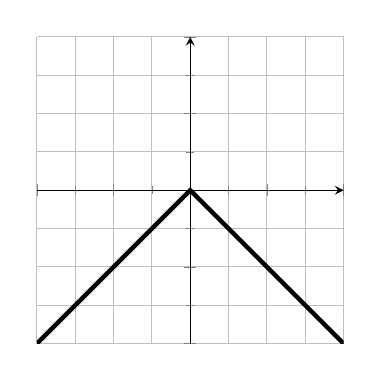
\begin{tikzpicture}
                \begin{axis}[
                    width=2.5in,
                    grid=both,
                    axis x line = middle,axis y line = middle,
                    axis equal image,
                    % xtick distance = 2, ytick distance = 2,
                    xmin = -4, xmax = 4,
                    ymin = -4, ymax = 4,
                    minor tick num = 1,
                    yticklabels={,,},
                    xticklabels={,,},
                    ]
                    \addplot[
                        no marks,
                        mark size = 0.1cm, ultra thick,
                        ] expression { -abs(x) };
                \end{axis}
            \end{tikzpicture}
        \end{minipage}
        \begin{minipage}{0.3\textwidth}
            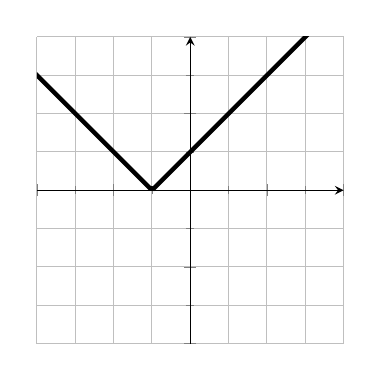
\begin{tikzpicture}
                \begin{axis}[
                    width=2.5in,
                    grid=both,
                    axis x line = middle,axis y line = middle,
                    axis equal image,
                    % xtick distance = 2, ytick distance = 2,
                    xmin = -4, xmax = 4,
                    ymin = -4, ymax = 4,
                    minor tick num = 1,
                    yticklabels={,,},
                    xticklabels={,,},
                    ]
                    \addplot[
                        no marks,
                        mark size = 0.1cm, ultra thick,
                        samples=100,
                        ] expression { abs(x+1) };
                \end{axis}
            \end{tikzpicture}
        \end{minipage}
        \begin{minipage}{0.3\textwidth}
            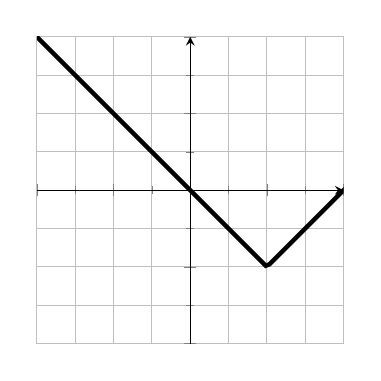
\begin{tikzpicture}
                \begin{axis}[
                    width=2.5in,
                    grid=both,
                    axis x line = middle,axis y line = middle,
                    axis equal image,
                    % xtick distance = 2, ytick distance = 2,
                    xmin = -4, xmax = 4,
                    ymin = -4, ymax = 4,
                    minor tick num = 1,
                    yticklabels={,,},
                    xticklabels={,,},
                    ]
                    \addplot[
                        no marks,
                        mark size = 0.1cm, ultra thick,
                        samples=100,
                        ] expression { abs(x-2)-2 };
                \end{axis}
            \end{tikzpicture}
        \end{minipage}
        \vspace{3in}
    \end{myExample}
\end{taggedblock}